\subsection*{\underline{طراحی بخش Front}}

برای طراحی بخش Front پروژه، هر صفحه را داخل یک Layout طراحی کردیم و با اسم خاص خودش ذخیره کردیم تا در آینده به بک‌اند متصل شود. 

برای فراخوانی Component های مختلف Material3 ، از آدرس 
$com.google.material*$
استفاده کردیم.

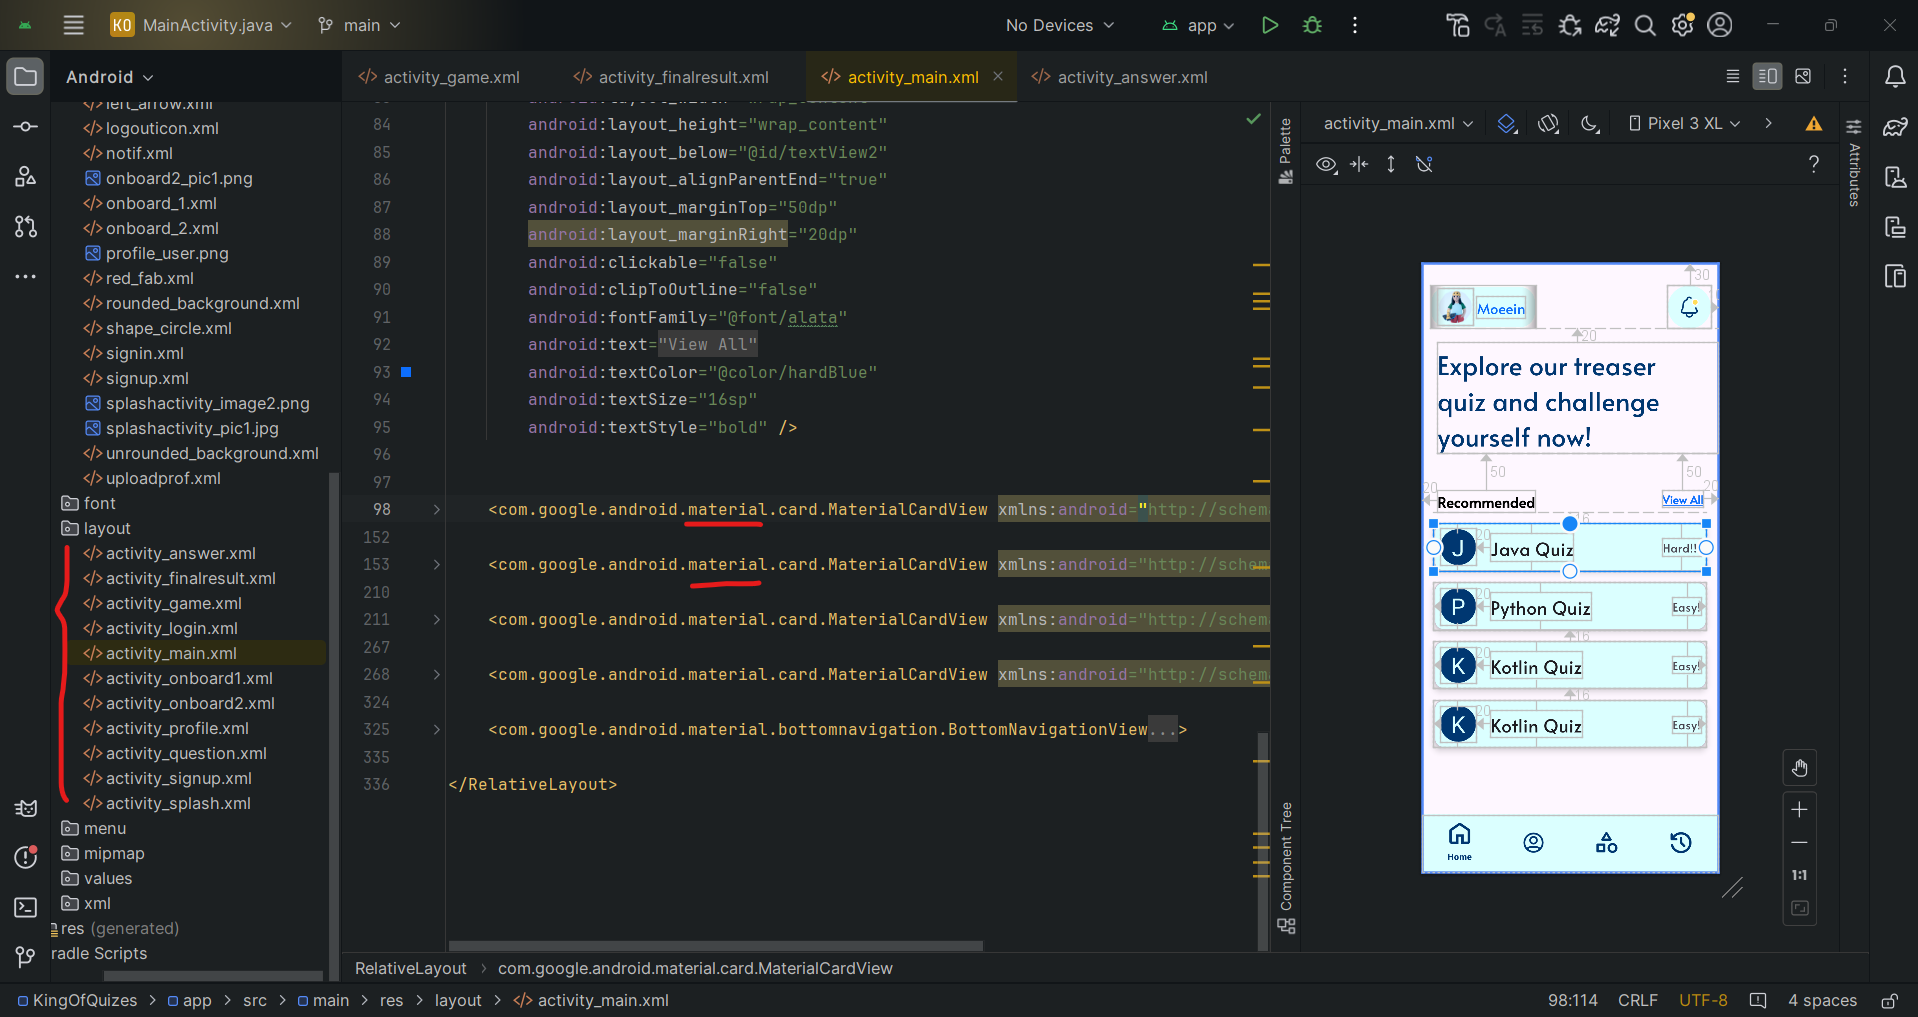
\includegraphics[width=1\linewidth]{screenshot001}


همچنین برای آسانی کار، رنگ‌های خاص پروژه خود را داخل بخش Colors.xml تعریف کردیم تا به آسانی در آینده آن‌ها را تغییر بدهیم.

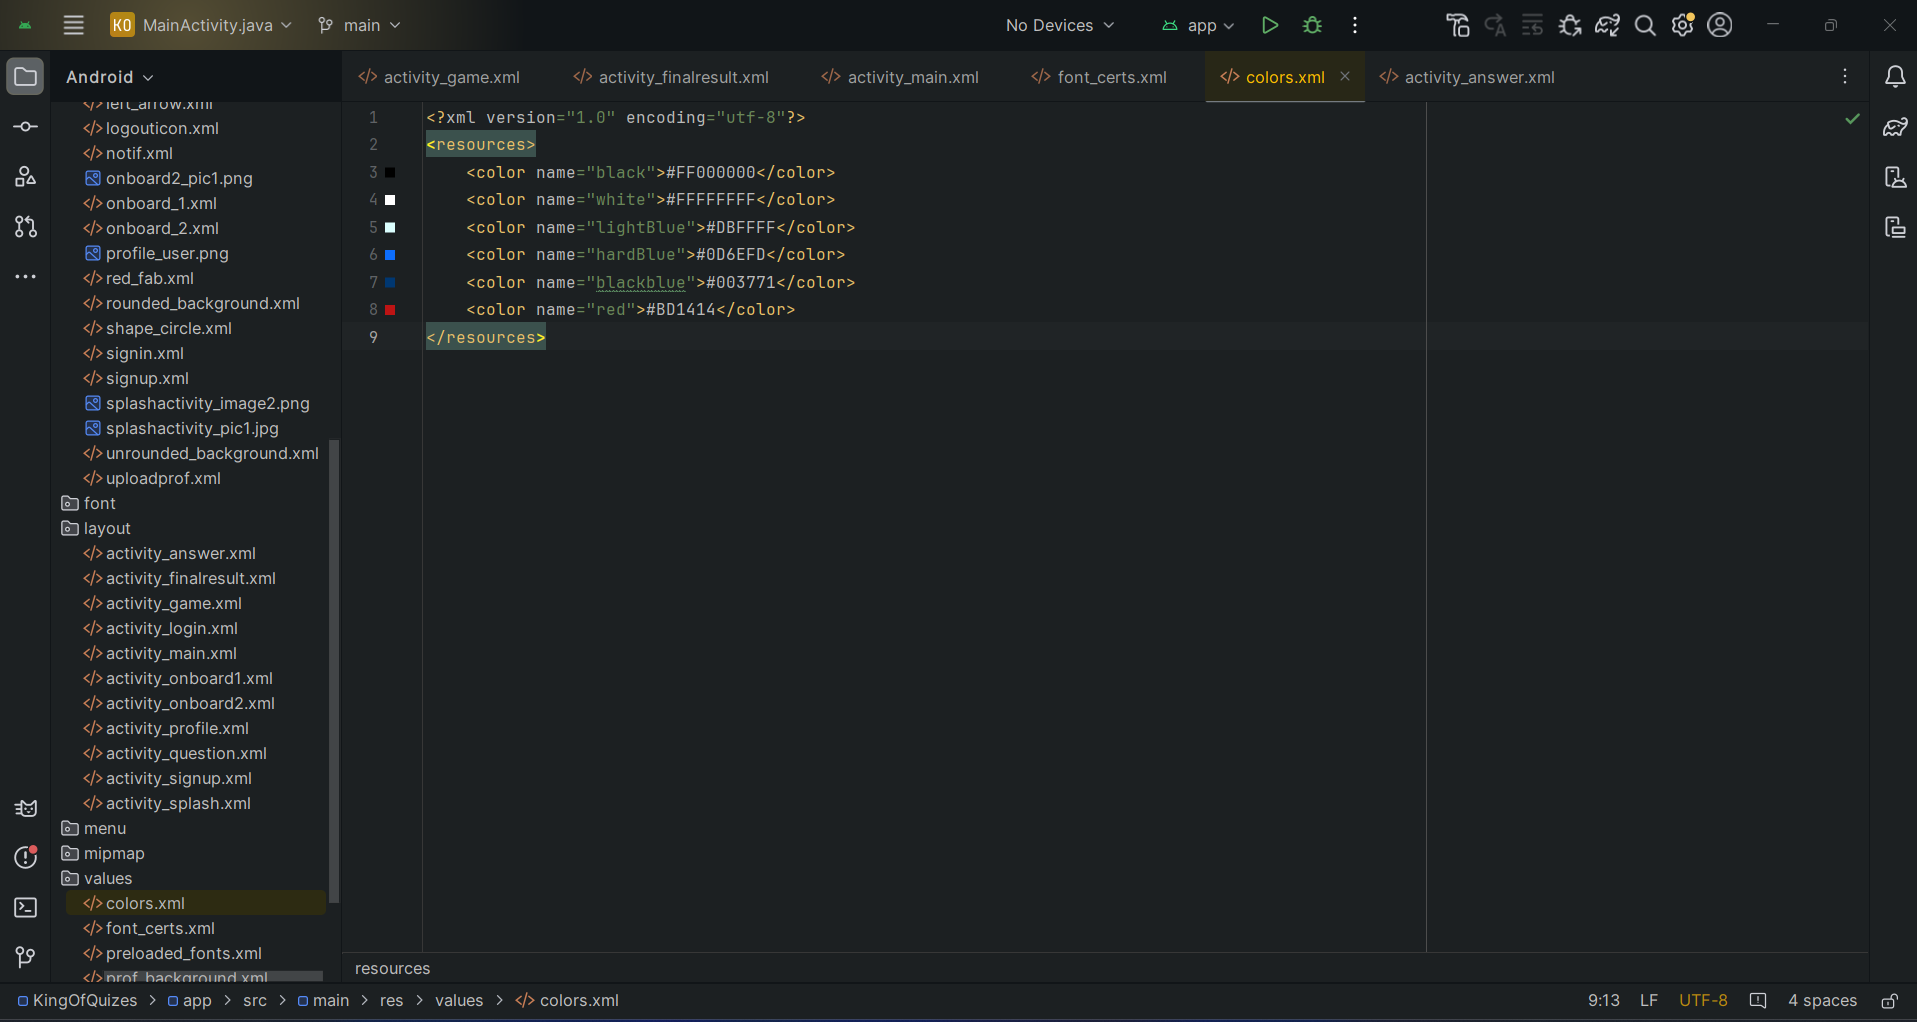
\includegraphics[width=1\linewidth]{screenshot002}

\pagebreak


آیکون های مورد استفاده در پروژه را به صورت svg داخل فیگما طراحی کردیم و سپس آن را از طریق 
$Import Vector$
به پوشه Drawable اضافه کردیم و داخل برنامه استفاده کردیم. مزیت این کار کم بودن لود و حجم تصاویر نسبت به حالت png است.

	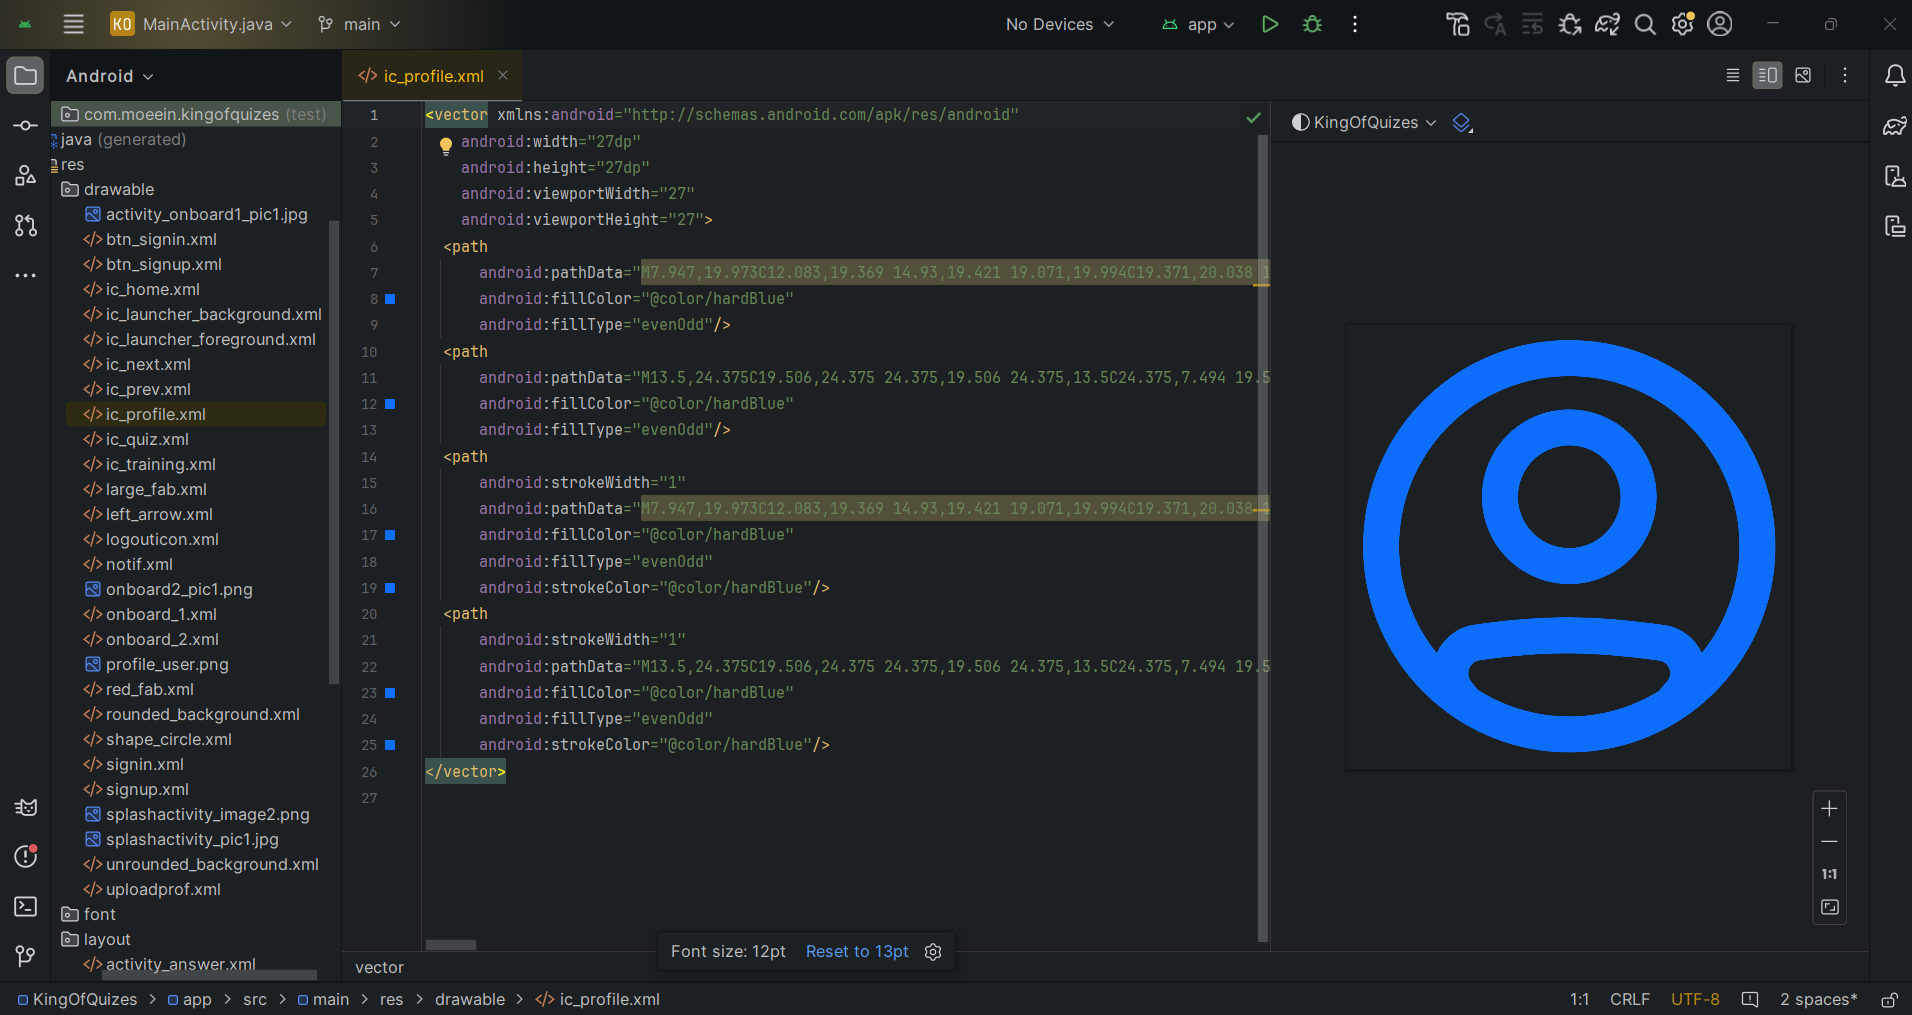
\includegraphics[width=1\linewidth]{screenshot003}


در آخر باید اشاره کنیم که داکیومنت های وبسایت $https://m3.material.io/$ خیلی به ما کمک کرد. هم برای استفاده از Component ها و هم در پیاده سازی منطق استفاده از این Component ها.



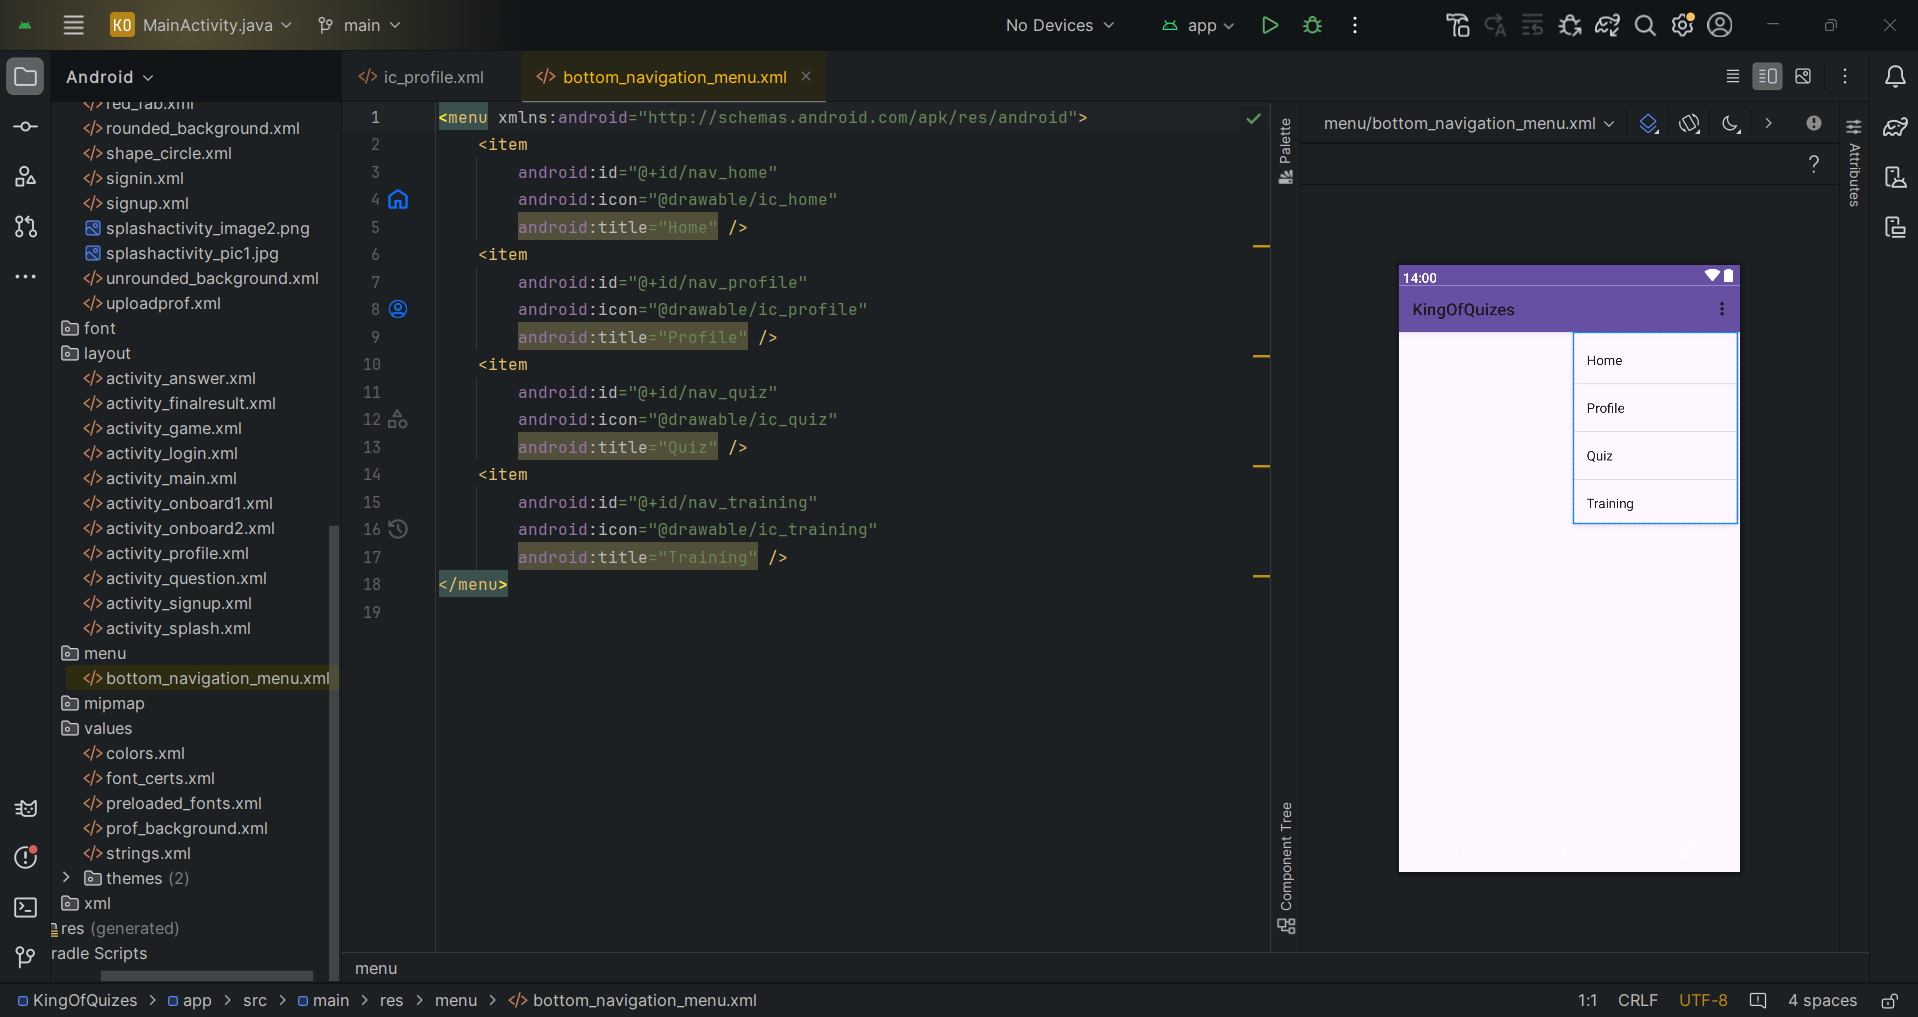
\includegraphics[width=1\linewidth]{screenshot005}

همچنین برای پیاده سازی NavBar موجود در منو اصلی مجبور شدیم که یک xml مربوط به menu داخل پوشه menu ایجاد کنیم و آبجکت های منو را داخلش تعریف کنیم و در آخر این فایل menu را به فوتر برنامه اضافه کنیم.








